\documentclass[10pt]{report}
\usepackage[utf8]{inputenc} % encodage du fichier
\usepackage[french]{babel} % document en francais
\usepackage[T1]{fontenc} % pour les caracteres accentues
\usepackage{geometry}
\geometry{a4paper, left=2.5cm, right=2.5cm, top=2.5cm, bottom=2.5cm}
\usepackage{Ressources/pseudocode}
\usepackage{mdframed}
\usepackage{xcolor}
\usepackage{minted}
\usepackage{multirow}
\usepackage{multicol}
\usepackage{array}
\usepackage{graphicx}  % Package pour l'inclusion d'images

\graphicspath{{Ressources/}}

%%definition de commandes
\newcommand{\octet}{\textbf{Octet}}
\newcommand{\codebinaire}{\textbf{CodeBinaire}}
\newcommand{\tabledecodage}{\textbf{TableDeCodage}}
\newcommand{\statistiques}{\textbf{Statistiques}}
\newcommand{\bit}{\textbf{Bit}}
\newcommand{\arbredehuffman}{\textbf{ArbreDeHuffman}}
\newcommand{\filedepriorite}{\textbf{FileDePriorite}}
\newcommand{\element}{\textbf{Element}}
\newcommand{\fichierbinaire}{\textbf{FichierBinaire}}

\begin{document}

	\tableofcontents

	\chapter{Introduction} 
        \section{Introdution}
	La compression de données est un domaine de recherche actif depuis de nombreuses années. Elle vise à réduire la taille des données en conservant le contenu original. La compression est utilisée dans de nombreuses applications, telles que le stockage de données, la transmission de données et le traitement des données.

	Il existe de nombreux algorithmes de compression différents. Les algorithmes de compression les plus courants sont les algorithmes de compression par perte et les algorithmes de compression sans perte.

	L'objectif de ce projet est de développer un algorithme de compression sans perte basé sur un arbre de Huffman et ensuite évaluer l'efficacité de l'algorithme de compression développé.
	
	Le rapport de ce projet sera présenter comme suis:
 
	\begin{enumerate}
		\item Présentation des TADs et des analyses descendantes;
		\item Conception préliminaire;
		\item Conception Détaillée.
		\item Code C et tests unitaires;
		\item Organisation et Travail de groupe;
		\item Conclusion.
	\end{enumerate}

    
    \chapter{Types Abstraits de Données}
        \section{Analyse : les TAD}
            \subsection{TAD Octet}
                \subsection{TAD Octet}

%\begin{mdframed}
\begin{tad}
    \tadNom{Octet}
    \tadDependances{\textbf{Bit}, \textbf{0..7}}
    \begin{tadOperations}{octetVersNaturel}
        \tadOperation{creerOctet}{\tadParams{\textbf{Bit},\textbf{Bit},\textbf{Bit},\textbf{Bit},\textbf{Bit},\textbf{Bit},\textbf{Bit},\textbf{Bit}}}{\textbf{Octet}}
        \tadOperation{obtenirIemeBit}{\tadParams{\textbf{Octet},\textbf{0..7}}}{\textbf{Bit}}
        \tadOperation{octetVersNaturel}{\textbf{Octet}}{\textbf{0..255}}    
    \end{tadOperations}

    \begin{tadAxiomes}
        \tadAxiome{obtenirIemeBit(creerOctet(b_0,b_1,b_2,b_3,b_4,b_5,b_6,b_7),0)= b_0}\\
        \textit{Note : on obtient $b_1$ pour l'indice 1, ... et $b_7$ pour l'indice 7}
    \end{tadAxiomes}
    
    \begin{tadSemantiques}{octetVersNaturel}
    	\tadSemantique{octetVersNaturel}{permet la conversion d'un nombre en base 2 (Octet) vers un nombre en base 10 (Naturel)}
    \end{tadSemantiques}

\end{tad}
%\end{mdframed}

            \subsection{TAD Statistiques}
                \begin{tad}
  \tadNom{Statistiques}
  \tadDependances{\octet}
  \begin{tadOperations}{obtenirElementEtDefiler}
  
    \tadOperation{statistiques}{}{\statistiques}
    \tadOperation{incrementerOccurrence}{\tadParams{\statistiques, \octet}}{\statistiques}
    \tadOperation{obtenirOccurrence}{\tadParams{\statistiques, \octet}}{\naturel}
    \tadOperation{fixerOccurrence}{\tadParams{\statistiques, \octet, \naturel}}{\statistiques}
  
    %\tadOperation{longueur}{FileDePriorite}{\naturel}
    
  \end{tadOperations}

  \begin{tadAxiomes}
        \tadAxiome{obtenirOccurrence(statistique(), o)=0}
        \tadAxiome{obtenirOccurrence(incrementerOccurrence(s,o), o) = obtenirOccurrence(s,o)+1}
 		\tadAxiome{obtenirOccurrence(fixerOccurrence(s, o, n), o) = n}
  \end{tadAxiomes}
  
  
  
\end{tad}
            \subsection{TAD FileDePriorite}
                \documentclass[10pt]{article}
\usepackage[utf8]{inputenc} % encodage du fichier
\usepackage[french]{babel} % document en francais
\usepackage[T1]{fontenc} % pour les caracteres accentues
\usepackage{geometry}
\geometry{a4paper, left=2.5cm, right=2.5cm, top=2.5cm, bottom=2.5cm}
\usepackage{pseudocode}
\usepackage{mdframed}

\begin{document}

%\begin{mdframed}
\begin{tad}
  \tadNom{FileDePriorite}
  \tadParametres{Element ($\forall e_1 \in Element, e_2 \in Element, e_1 \neq e_2 \Rightarrow e_1 < e_2 \textit{ ou } e_1 > e_2$)}
  \tadDependances{\booleen}
  \begin{tadOperations}{obtenirElementEtDefiler}
  
    \tadOperation{fileDePriorite}{}{FileDePriorite}
    \tadOperation{estVide}{FileDePriorite}{\booleen}
    \tadOperation{enfiler}{\tadParams{FileDePriorite, Element}}{FileDePriorite}
    \tadOperationAvecPreconditions{obtenirElementEtDefiler}{FileDePriorite}{\tadParams{FileDePriorite, Element}}
    %\tadOperation{longueur}{FileDePriorite}{\naturel}
    
  \end{tadOperations}
  \parbox{\linewidth}{\raggedright
      \begin{tadAxiomes}
          \tadAxiome{estVide(fileDePriorite())}
          \tadAxiome{non(estVide(enfiler(f, e)))}
          \tadAxiome{obtenirElementEtDefiler(enfiler(fileDePriorite(),e)) = fileDePriorite(),e}
          \tadAxiome{e \leq obtenirElementEtDefiler(f)[2] \Rightarrow obtenirElementEtDefiler(enfiler(f,e)) = f,e}
          \tadAxiome{e > obtenirElementEtDefiler(f)[2] \Rightarrow obtenirElementEtDefiler(enfiler(f,e)) = enfiler(obtenirElementEtDefiler(f)[1],e),obtenirElementEtDefiler(f)[2]}
      \end{tadAxiomes}
  }
  
  \begin{tadPreconditions}{obtenirElementEtDefiler(f)}
    \tadPrecondition{obtenirElementEtDefiler(f)}{non(estVide(f))}
  \end{tadPreconditions}
  
\end{tad}
%\end{mdframed}




\end{document}

            \subsection{TAD ArbreDeHuffman}
                \documentclass[10pt]{article}
\usepackage[utf8]{inputenc} % encodage du fichier
\usepackage[french]{babel} % document en francais
\usepackage[T1]{fontenc} % pour les caracteres accentues
\usepackage{geometry}
\geometry{a4paper, left=2.5cm, right=2.5cm, top=2.5cm, bottom=2.5cm}
\usepackage{pseudocode}
\usepackage{mdframed}

\begin{document}

%\begin{mdframed}
\begin{tad}
  \tadNom{ArbreDeHuffman}
  \tadParametres{Element, Frequence}
  \tadDependances{\booleen}
  \begin{tadOperations}{obtenirFilsGauche}
  
    \tadOperation{arbreDeHuffman}{\tadParams{Element, Frequence}}{ArbreDeHuffman}
    \tadOperation{ajouterRacine}{\tadParams{ArbreDeHuffman, ArbreDeHuffman}}{ArbreDeHuffman}
    \tadOperation{estUneFeuille}{ArbreDeHuffman}{\booleen}
    \tadOperationAvecPreconditions{obtenirElement}{ArbreDeHuffman}{Element}
    \tadOperation{obtenirFrequence}{ArbreDeHuffman}{Frequence}
    \tadOperationAvecPreconditions{obtenirFilsGauche}{ArbreDeHuffman}{ArbreDeHuffman}
    \tadOperationAvecPreconditions{obtenirFilsDroit}{ArbreDeHuffman}{ArbreDeHuffman}
    
  \end{tadOperations}
  \parbox{\linewidth}{\raggedright
      \begin{tadAxiomes}
            \tadAxiome{estUneFeuille(arbreDeHuffman(e,f))}
            \tadAxiome{non(estUneFeuille(ajouterRacine(a_g,a_d)))}
            \tadAxiome{obtenirElement(arbreDeHuffman(e,f)) = e}
            \tadAxiome{obtenirFrequence(arbreDeHuffman(e,f)) = f}
            \tadAxiome{obtenirFrequence(ajouterRacine(a_g,a_d)) = obtenirFrequence(a_g) + obtenirFrequence(a_d)}
            \tadAxiome{obtenirFilsGauche(ajouterRacine(a_g,a_d)) = a_g}
            \tadAxiome{obtenirFilsDroit(ajouterRacine(a_g,a_d)) = a_d}
      \end{tadAxiomes}
  }
  
  \begin{tadPreconditions}{obtenirFilsGauche(a)}
    \tadPrecondition{obtenirElement(a)}{estUneFeuille(a)}
    \tadPrecondition{obtenirFilsGauche(a)}{non(estUneFeuille(a))}
    \tadPrecondition{obtenirFilsDroit(a)}{non(estUneFeuille(a))}
  \end{tadPreconditions}
  
\end{tad}
%\end{mdframed}

\end{document}

            \subsection{TAD CodeBinaire}
                \begin{tad}
  \tadNom{CodeBinaire}
  \tadDependances{\textbf{Octet}, \naturel, \textbf{Bit}}
  \begin{tadOperations}{obtenirLongueur}
  
    \tadOperation{creerCodeBinaire}{\bit}{\codebinaire}
    \tadOperation{ajouterBit}{\tadParams{\codebinaire, \bit}}{\codebinaire}
    \tadOperationAvecPreconditions{obtenirIemeBit}{\tadParams{\codebinaire, \naturel}}{\bit}
    \tadOperation{obtenirLongueur}{\codebinaire}{\naturel}
     
  \end{tadOperations}

  \begin{tadPreconditions}{obtenirIemeBit(cb, i)}
    \tadPrecondition{obtenirIemeBit(cb, i)}{i < obtenirLongueur(cb)}
  \end{tadPreconditions}

  \begin{tadAxiomes}	

    \tadAxiome{obtenirLongueur(creerCodeBinaire(b)) = 1}
    \tadAxiome{obtenirLongueur(ajouterBit(cb, b)) = obtenirLongueur(cb) + 1}

  \end{tadAxiomes}
  
  \begin{tadSemantiques}{obtenirIemeBit}

    \tadSemantique{ajouterBit}{Ajoute le bit en question à la fin du CodeBinaire}
    \tadSemantique{obtenirIemeBit}{Retourne le bit à la position i du CodeBinaire (0 étant la position du premier bit)}
    
  \end{tadSemantiques}
\end{tad}
            \subsection{TAD TableDeCodage}
                \begin{tad}
    \tadNom{TableDeCodage}
    \tadDependances{\textbf{Octet}, \booleen, \textbf{CodeBinaire}}
    \begin{tadOperations}{octetVersCodeBinaire}
        \tadOperation{creerTableCodage}{}{\textbf{TableDeCodage}}
        \tadOperationAvecPreconditions{ajouterCodage}{\tadParams{\textbf{TableDeCodage},\textbf{Octet},\textbf{CodeBinaire}}}{\textbf{TableDeCodage}}
        \tadOperation{octetPresent}{\tadParams{\textbf{TableDeCodage},\textbf{Octet}}}{\textbf{\booleen}}
        \tadOperationAvecPreconditions{octetVersCodeBinaire}{\tadParams{\textbf{TableDeCodage},\textbf{Octet}}}{\textbf{CodeBinaire}}
    \end{tadOperations}

    \begin{tadPreconditions}{octetVersCodeBinaire(t, codeBinaire)}
        \tadPrecondition{ajouterCodage(t,octet,codeBinaire)}{non(octetPresent(t, octet))}
        \tadPrecondition{octetVersCodeBinaire(t, octet)}{octetPresent(t, octet)}
    \end{tadPreconditions}

    \begin{tadAxiomes}
    	\tadAxiome{octetPresent(ajouterCodage(t, octet, codeBinaire), octet)}
    	\tadAxiome{non(octetPresent(creerTableCodage(), octet))}
        \tadAxiome{octetVersCodeBinaire(ajouterCodage(t, octet, codeBinaire), octet)=codeBinaire}
    \end{tadAxiomes}
    

\end{tad}


        \newpage
        \section{Conception Préliminaire}
            \subsection{Signatures et fonctions de Octet}
                \subsection{Conception préliminaire : Octet}

\begin{algorithme}
    \signatureFonction{creerOctet}
    {b0, b1, b2, b3, b4, b5, b6, b7 : \textbf{Bit}}
    {\textbf{Octet}}
    {}
    \signatureFonction{obtenirIemeBit}
    {o : \textbf{Octet}, b : \textbf{0..7}}
    {\textbf{Bit}}
    {}
    \signatureFonction{octetVersNaturel}
    {o : \textbf{Octet}}
    {\textbf{0..255}}
    {}
    \signatureFonction{naturelVersOctet}
    {n : \textbf{0..255}}
    {\textbf{Octet}}
    {}
\end{algorithme}

            \subsection{Signatures et fonctions de Statistiques}
                \subsection{Conception préliminaire : Statistiques}

\begin{algorithme}
    \signatureFonction{statistiques}
    {}{\textbf{Statistiques}}
    {}
    \signatureProcedure{incrementerOccurence}
    {\paramEntreeSortie{s : \textbf{Statistiques}}, o : \paramEntree{\textbf{Octet}}}
    {}
    \signatureFonction{obtenirOccurence}
    {o : \textbf{Octet}, s : \textbf{Statistiques}}
    {\naturel}
    {}
\end{algorithme}
            \subsection{Signatures et fonctions de FileDePriorite}
                \begin{algorithme}
    \signatureFonction{fileDePriorite}{}{FileDePriorite}{}
    \signatureFonction{estVide}{fdp : FileDePriorite}{Booléen}{}
    \signatureProcedure{enfiler}{E/S fdp : FileDePriorite, E e : Element}{}
    \signatureProcedure{obtenirElementEtDefiler}{E/S fdp : FileDePriorite, S Element}{non(estVide(fdp))}
\end{algorithme}
            \subsection{Signatures et fonctions de ArbreDeHuffman}
                \subsection{Conception préliminaire : ArbreDeHuffman}

\begin{algorithme}

    \signatureFonction{arbreDeHuffman}
    {o : \textbf{Octet}, n : \textbf{Naturel}}
    {\textbf{ArbreDeHuffman}}{}
    \signatureFonction{fusionner}{ag : ArbreDeHuffman, ad : ArbreDeHuffman} {\textbf{ArbreDeHuffman}}{}
    
    \signatureFonction{estUneFeuille}{a: ArbreDeHuffman}
    {\textbf{Booleen}}{}
    \signatureFonction{obtenirOctect}
    {a: ArbreDeHuffman}
    {\textbf{Octet}}{estUneFeuille(a)}
    \signatureFonction{obtenirFrequence}
    {a: ArbreDeHuffman}
    {\textbf{Naturel}}{}
     \signatureFonction{obtenirFilsGauche}
    {a: ArbreDeHuffman}
    {\textbf{ArbreDeHuffman}}{non(estUneFeuille(a))}
      \signatureFonction{obtenirFilsDroit}
    {a: ArbreDeHuffman}
    {\textbf{ArbreDeHuffman}}{non(estUneFeuille(a))}
    
\end{algorithme}

            \subsection{Signatures et fonctions de CodeBinaire}
                \begin{algorithme}
    \signatureFonction{creerCodeBinaire}{b : \bit}{\codebinaire}{}
    \signatureProcedure{ajouterBit}{\paramEntreeSortie{cb : \codebinaire}, \paramEntree{b : \bit}}{}
    \signatureFonction{obtenirIemeBit}{cb : \codebinaire, i : \naturel}{\bit}{i < obtenirLongueur(cb)}
    \signatureFonction{obtenirLongueur}{cb : \codebinaire}{\naturel}{}
\end{algorithme}

            \subsection{Signatures et fonctions de TableDeCodage}
                \begin{algorithme}
    \signatureFonction{creerTableCodage}{}{TableDeCodage}{}
    \signatureProcedure{ajouterCodage}{E/S tdc : TableDeCodage, E o : octet, E cb:Codebinaire}{}
     \signatureFonction{OctetPresent}{tdc : TableDeCodage,o :octet}{Booleen}{}
    \signatureFonction{OctetVersCodeBinaire}{tdc : TableDeCodage,o :octet}{CodeBinaire}{octetPresent(t,octet)}
   
\end{algorithme}

        \newpage
        \section{Conception Détaillée}
            \textbf{// Dans le but de simplifier la conception détaillée ainsi que le développement, nous considérons bitA0 = 0 et bitA1 = 1. Nous pouvons ainsi utiliser le type Bit comme un naturel. Cela permet d'éviter des instructions conditionnelles répétitives et coûteuses bien que triviales.}
            \subsection{Algorithmes de Octet}
                \begin{algorithme}
    \type{Octet}{\textbf{0..255}}
    \\
    \fonction{creerOctet}
    {b7, b6, b5, b4, b3, b2, b1, b0 : \textbf{Bit}}
    {\textbf{Octet}}
    {}
    {o : \textbf{Octet}}
    {  		
        \affecter{o}{b0 + b1*2 + b2*2\^{}2 + b3*2\^{}3 + b4*2\^{}4 + b5*2\^{}5 + b6*2\^{}6 + b7*2\^{}7}
        \retourner{o}
    }
    \\
    \fonction{obtenirIemeBit}
    {o : \textbf{Octet}, b : \textbf{0..7}}
    {\textbf{Bit}}
    {}
    {}
    {
        \retourner{(o \textbf{div} 2\^{}b) \textbf{mod} 2}
    }
 	\\
    \fonction{octetVersNaturel}
    {o : \textbf{Octet}}
    {\textbf{0..255}}
    {}
    {}
	{   
    {
       \retourner{o}
    }
    }
    \\
    \fonction{naturelVersOctet}
    {n : \textbf{0..255}}
    {\textbf{Octet}}
    {}
    {}
	{   
    {
       \retourner{n}
    }
    }
\end{algorithme}

            \subsection{Algorithmes de Statistiques}
                \begin{algorithme}
    \type{Statistiques}{\tableauUneDimension{0..255}{de }{\naturel}}
    \\
    \fonction{statistiques}{}{\statistiques}
    {}
    {s : \statistiques}
    {
        \pour{octet}{ 0}{255}{}{
            \affecter{s[octet]}{0}
        }
        \retourner{s}
    }
    \\
    \procedure{incrementerOccurrence}{\paramEntreeSortie{s : \statistiques}, \paramEntree{o : \octet}}
    {}
    {}
    {
    	\affecter{s[octetVersNaturel(o)]}{s[octetVersNaturel(o)] + 1}
    }
    \\
    \fonction{obtenirOccurrence}{s : \statistiques, o : \octet}{\textbf{Naturel}}
    {}
    {}
    {
    	\retourner{s[octetVersNaturel(o)]}
    }
    \procedure{fixerOccurrence}{\paramEntreeSortie{s : \statistiques}, \paramEntree{o : \octet, n : \naturel}}
    {}
    {}
    {
    	\affecter{s[octetVersNaturel(o)]}{n}
    }
\end{algorithme}
            \subsection{Algorithmes de FileDePriorite}
                \subsection{File de Priorité}
\begin{algorithme}
    \procedure{enfiler}{\paramEntreeSortie{file : \textbf{FileDePriorite}}, \paramEntree{e : \textbf{Element}}}{}
    {temp : \textbf{FileDePriorite}}
    {
         \sialorssinon{estVide(file) ou e $\leq$ file\motclefDereferencer .element}
         {
            \affecter{temp}{file}
            \instruction{\allouer{file}}
            \affecter{file\motclefDereferencer .element}{e}
            \affecter{file\motclefDereferencer .fileSuivante}{temp}
         }
         {
            \instruction{\textbf{enfiler}(file\motclefDereferencer .fileSuivante, e)}{}
         }
    }
\end{algorithme}

\bigbreak
\begin{algorithme}
    \procedure{obtenirElementEtDefiler}{\paramEntreeSortie{file : \textbf{FileDePriorite}, \paramSortie{e : \textbf{Element}}}}{non(estVide(file))}
    {temp : \textbf{FileDePriorite}}
    {
        \affecter{e}{file\motclefDereferencer .element}
        \affecter{temp}{file}
        \affecter{file}{temp\motclefDereferencer .listeSuivante}
        \instruction{\desallouer{temp}}
    }
\end{algorithme}

\bigbreak
\begin{algorithme}
    \fonction{fileDePriorite}{}{\textbf{FileDePriorite}}{}
    {}
    {
        \retourner{\textbf{NIL}}
    }
\end{algorithme}

\bigbreak
\begin{algorithme}
    \fonction{estVide}{file : \textbf{FileDePriorite}}{\booleen}{}
    {}
    {
        \retourner{file = \textbf{NIL}}
    }
\end{algorithme}
            \subsection{Algorithmes de ArbreDeHuffman}
                \begin{algorithme}
	\type{ArbreDeHuffman}{$\widehat{}$ Noeud}
	\begin{enregistrement}{Noeud}
		\champEnregistrement{octet}{\octet}
		\champEnregistrement{frequence}{\naturel}
		\champEnregistrement{estUneFeuille}{\booleen}
		\champEnregistrement{filsGauche}{\arbredehuffman}
		\champEnregistrement{filsDroit}{\arbredehuffman}
	\end{enregistrement}
	\\
    \fonction{arbreDeHuffman}{o : \octet, f : \naturel}{\arbredehuffman}{}
    {a : ArbreDeHuffman}
    {
        \instruction{\allouer{a}}
        \affecter{a\motclefDereferencer .octet}{o}
        \affecter{a\motclefDereferencer .frequence}{f}
        \affecter{a\motclefDereferencer .estUneFeuille}{\textbf{Vrai}}
        \affecter{a\motclefDereferencer .filsGauche}{\textbf{NIL}}
        \affecter{a\motclefDereferencer .filsDroit}{\textbf{NIL}}
        \retourner{a}
    }
	\\
    \fonction{fusionner}{$a_g$, $a_d$ : \arbredehuffman}{\arbredehuffman}{}
    {racine : \arbredehuffman}
    {
        \instruction{\allouer{racine}}
        \affecter{racine\motclefDereferencer .filsGauche}{$a_g$}
        \affecter{racine\motclefDereferencer .filsDroit}{$a_d$}
        \affecter{racine\motclefDereferencer .estUneFeuille}{\textbf{Faux}}
        \affecter{racine\motclefDereferencer .frequence}{obtenirFrequence($a_g$) + obtenirFrequence($a_d$)}
        \retourner{racine}
    }
	\\
    \fonction{estUneFeuille}{a : \arbredehuffman}{\booleen}{}
    {}
    {
        \retourner{a\motclefDereferencer .estUneFeuille}
    }
	\\
    \fonction{obtenirOctet}{a : \arbredehuffman}{\octet}{estUneFeuille(a)}
    {}
    {
        \retourner{a\motclefDereferencer .octet}
    }
	\\
    \fonction{obtenirFrequence}{a : \arbredehuffman}{\naturel}{}
    {}
    {
        \retourner{a\motclefDereferencer .frequence}
    }
	\\
    \fonction{obtenirFilsGauche}{a : \arbredehuffman}{\arbredehuffman}{non(estUneFeuille(a))}
    {}
    {
        \retourner{a\motclefDereferencer .filsGauche}
    }
	\\
    \fonction{obtenirFilsDroit}{a : \arbredehuffman}{\arbredehuffman}{non(estUneFeuille(a))}
    {}
    {
        \retourner{a\motclefDereferencer .filsDroit}
    }
    \\
    \procedure{liberer}{\paramEntree{arbre : \arbredehuffman}}{}{}
    {
        \sialors{non(estUneFeuille(arbre))}
        {
            \instruction{liberer(obtenirFilsGauche(arbre))}
            \instruction{liberer(obtenirFilsDroit(arbre))}
        }
        \instruction{\textbf{desallouer}(arbre)}
    }
\end{algorithme}

            \subsection{Algorithmes de CodeBinaire}
                \begin{algorithme}
    \begin{enregistrement}{CodeBinaire}
        \champEnregistrement{codeBinaire}{\textbf{Naturel}}
        \champEnregistrement{nbBits}{\textbf{Naturel}}
    \end{enregistrement}
    \\
    \fonction{creeCodeBinaire}
    {b: \textbf{Naturel}}
    {\textbf{CodeBinaire}}
    {}
    {cb : \textbf{CodeBinaire}}
    {  		
    	\affecter{cb.codebinaire}{b}
    	\affecter{cb.nbBits}{1}
        \retourner{cb}
    }
    \\
    \fonction{obtenirIemeBit}
    {cb : \textbf{CodeBinaire}, i: \textbf{0..7}}
    {\textbf{Bit}}
    {}
    {}
    {
        \retourner{cb.codeBinaire/$2^{i}$}
    }
 	\\
    \fonction{obtenirLongueur}{cb : CodeBinaire}
    {\textbf{Naturel}}
    {}
    {}
    {
       \retourner{cb.bits}
    }
    \\
     \procedure{ajouterBit}{E/S cb : CodeBinaire, E b : bit}
    {}
    {}
    {
       \affecter {cb.codebinaire}{cb.codebinaire + (b*$2^{cb.nbBits}$)}
	    \affecter {cb.nbElements}{obtenirLongueur(cd)+1}
    }
\end{algorithme}

            \subsection{Algorithmes de TableDeCodage}
                \section{Conception Détaillée : TableDeCodage}

\newcommand{\octet}{\textbf{Octet}}
\newcommand{\codebinaire}{\textbf{CodeBinaire}}
\newcommand{\tabledecodage}{\textbf{TableDeCodage}}

\begin{algorithme}
    \type{TableDeCodage}{Dictionnaire<Octet,CodeBinaire>}
    \\
    \fonction{creerTableCodage}{o : \octet, cb : \codebinaire}{\tabledecodage}
    {}
    {tdc : \tabledecodage}
    {
        \affecter{tdc}{dictionnaire()}
        \instruction{ajouter(tdc,o,cb)}
        \retourner{tdc}
    }
    \\
    \procedure{ajouterCodage}{tdc : \tabledecodage, o : \octet, cb : \codebinaire}
    {non(octetPresent(t, octet))}
    {}
    {
        \instruction{ajouter(tdc,o,cb)}
    }
    \\
    \fonction{octetVersCodeBinaire}{tdc : \tabledecodage, o : \octet}{\codebinaire}
    {octetPresent(t, octet)}
    {}
    {
        \retourner{obtenirValeur(tdc,o)}
    }
    \\
    \fonction{octetPresent}{tdc : \tabledecodage, o : \octet}{\booleen}
    {}
    {}
    {
        \retourner{estPresent(tdc,o)}
    }
\end{algorithme}

    \chapter{Compression}
        \section{Analyse descendante}

\newpage
\section{Conception Préliminaire}
    \begin{algorithme}
    \signatureProcedure{obtenirStatistiquesEtTailleFichier}{\paramEntreeSortie{f : \fichierbinaire}, \paramSortie{s : \statistiques, taille : \naturel}}{estOuvert(f) et (mode(f) $=$ lecture)}
\end{algorithme}
    \begin{algorithme}
    \signatureFonction{construireFileDePriorite}{s : \statistiques}{\filedepriorite}{}
\end{algorithme}
    \begin{algorithme}
    \signatureFonction{construireArbreDeHufmman}{s : \statistiques}{\arbredehuffman}{}
\end{algorithme}
    \begin{algorithme}
    \signatureProcedure{obtenirTableDeCodageRecursif}{\paramEntreeSortie{tdc : \tabledecodage}, \paramEntree{a : \arbredehuffman, cb : \codebinaire}}{}
    \signatureFonction{obtenirTableDeCodage}{a : \arbredehuffman}{\tabledecodage}{non(estUneFeuille(a))}
\end{algorithme}
    \begin{algorithme}
    \signatureProcedure{ecrireIdentifiant}{\paramEntreeSortie{fb : \fichierbinaire}}{}
    \signatureProcedure{ecrireTailleFichier}{\paramEntreeSortie{fb : \fichierbinaire}, \paramEntree{taillefb : \naturel}}{}
    \signatureProcedure{ecrireStatistiques}{\paramEntreeSortie{fb : \fichierbinaire}, \paramEntree{s : \statistiques}}{}
\end{algorithme}
    \begin{algorithme}
    \signatureFonction{codeBinaireEnOctet}{cb : \codebinaire}{\octet}{}
\end{algorithme}
    \begin{algorithme}
    \signatureProcedure{concatenerCodeBinaireDansFichier}{\paramEntreeSortie{cbtemp : \codebinaire},\paramEntree{cb : \codebinaire},\paramEntreeSortie{fbCompresse : \fichierbinaire}}{}
\end{algorithme}
    \begin{algorithme}
    \signatureFonction{encoder}{fb : \fichierbinaire, tdc : \tabledecodage}{\fichierbinaire}{}
\end{algorithme}
    \begin{algorithme}
    \signatureProcedure{compresser}{\paramEntreeSortie{f : \fichierbinaire}, \paramSortie{fCompresse : \fichierbinaire}}{}
\end{algorithme}

\newpage
\section{Conception Détaillée}
    \begin{algorithme}
    \procedure{obtenirStatistiquesEtTailleFichier}{\paramEntreeSortie{f : \fichierbinaire}, \paramSortie{s : \statistiques, taille : \naturel}}{}
    {s : \statistiques}
    {
        \sialors{estOuvert(f)}
        {
            \instruction{fermer(f)}
        }
        \instruction{ouvrir(f, lecture)} 
        \\
        \commentaire{Les instructions ci-dessus correspondent à une réinitialisation du curseur en tête de fichier.}
        \affecter{s}{statistiques()}
        \affecter{taille}{0}
        \tantque{non(finFichier(f))}
        {
            \instruction{incrementerOccurence(s, lireOctet(f))} 
            \affecter{taille}{taille + 1}   
        }
    }
\end{algorithme}
    \begin{algorithme}
    \fonction{construireFileDePriorite}{s : \statistiques}{\filedepriorite}{}
    {fdp : \filedepriorite, octet : \octet, occurence : \naturel}
    {
        \affecter{fdp}{fileDePriorite()}
        \pour{o}{ 0}{255}{}
        {
            \affecter{octet}{naturelVersOctet(o)}
            \affecter{occurence}{obtenirOccurence(s, octet)}
            \sialors{occurence > 0}{
                \instruction{enfiler(fdp, arbreDeHuffman(octet, occurence))}
            }
        }
        \retourner{fdp}
    }
\end{algorithme}
    \begin{algorithme}
	\fonction{construireArbreDeHuffman}{s : \statistiques}{\arbredehuffman}{}
	{fdp : \filedepriorite, dernierElement : \booleen, a1, a2, aFusion : \arbredehuffman}
    {
    	\affecter{fdp}{construireFileDePriorite(s)}
    	\affecter{dernierElement}{\textbf{Faux}}
    	\tantque{non(dernierElement)}
    	{
    		\instruction{obtenirElementEtDefiler(fdp, a1)}
    		\sialorssinon{estVide(fdp)}
    		{
    			\affecter{dernierElement}{\textbf{Vrai}}
    		}
    		{
    			\instruction{obtenirElementEtDefiler(fdp, a2)}
    			\affecter{aFusion}{fusionner(a1, a2)}
    			\instruction{enfiler(fdp, aFusion)}
    		}
    	}
    	\retourner{a1}
    }
\end{algorithme}
    \begin{algorithme}
    \procedure{obtenirTableDeCodageRecursif}{\paramEntree{a : \arbredehuffman}, \paramEntreeSortie{tdc : \tabledecodage, cb : \codebinaire}}
    {}
    {cbCopie : \codebinaire}
    {
        \sialorssinon{estUneFeuille(a)}
        {
            \instruction{ajouterCodage(tdc, cb)}
        }
        {
            \affecter{cbCopie}{cb}
            \instruction{ajouterBit(cbCopie, bitA0)}
            \instruction{obtenirTableDeCodageRecursif(obtenirFilsGauche(a), tdc, cbCopie)}
            \instruction{ajouterBit(cb, bitA1)}
            \instruction{obtenirTableDeCodageRecursif(obtenirFilsDroit(a), tdc, cb)}
        }
    }
    
    \fonction{obtenirTableDeCodage}{a : \arbredehuffman}{\tabledecodage}
    {}
    {tdc : \tabledecodage}
    {
        \affecter{tdc}{creerTableDeCodage()}
        \affecter{cbGauche}{creerCodeBinaire(bitA0)}
        \affecter{cbGauche}{creerCodeBinaire(bitA1)}
        \instruction{obtenirTableDeCodageRecursif(obtenirFilsGauche(a),tdc,cbGauche)}
        \instruction{obtenirTableDeCodageRecursif(obtenirFilsDroit(a),tdc,cbDroit)}
        \retourner{tdc}
    }
\end{algorithme}
    \begin{algorithme}
    \procedure{ecrireIdentifiant}{\paramEntreeSortie{fb : \fichierbinaire}}{}
    {}
    {
    	 \instruction{ecrireoctet(fb,creeoctet(0,0,0,0,0,0,1,1)}
         \instruction{ecrireoctet(fb,creeoctet(1,1,1,0,1,0,0,0)}
    }
    \procedure{ecrireStatistique}{\paramEntreeSortie{fb : \fichierbinaire},\paramEntree{s : \statistiques}}{}{}
    {
    	\instruction{ecrireoctet(fb)}
    }
    
    
     \procedure{ecrireTailleFichier}{\paramEntreeSortie{fb : \fichierbinaire},\paramEntree{taillefb : Naturel}}{}{}{
     \instruction{ecrireoctet(naturelVersOctet(taillefb),fb)}
     }
\end{algorithme}
    \begin{algorithme}
     \fonction{codeBinaireEnOctet}{cb: \fichierbinaire}{\octet}
    {obtenirLongueur(cb) $=$ 8}
    {}
    {        
        \retourner{creerOctet(obtenirIemeBit(cb,7), obtenirIemeBit(cb, 6), obtenirIemeBit(cb, 5), obtenirIemeBit(cb, 4),  obtenirIemeBit(cb, 3), obtenirIemeBit(cb, 2), obtenirIemeBit(cb, 1), obtenirIemeBit(cb, 0))}
    }
\end{algorithme}
    	    			  			
    	    			  						   
    \begin{algorithme}
     \procedure{concatenerCodeBinaireDansFichier}{\paramEntreeSortie{cbtemp : \codebinaire},\paramEntree{cb : \codebinaire},\paramEntreeSortie{fbCompresse : \fichierbinaire}}
    {}
    { i,j, tailleCbTemp, taillecb : Entier, o : \octet}
    {
        		\sialors{obtenirLongeur(cbtemp) = 8}
				{											
					\affecter{cbtemp}{cb}
				}
				\affecter{tailleCbTemp}{obtenirLongeur(cbtemp)}
        		\affecter{tailleCb}{obtenirLongeur(cb)}
				\affecter{tailleTotale}{tailleCbTemp + tailleCb}
        		\sialorssinon{tailleTotale $>$ 8}
        		{		
        			\pour{i}{0}{7 $-$ tailleCbTemp}{}
        			{
        				\instruction{ajouterBit(cbtemp,obtenirIemeBit(cb,i))}
					}    											
					\instruction{ecrireOctet(fbCompresse, codeBinaireEnOctet(cb))}
					\\
        			\affecter{cbtemp}{creeCodeBinaire(obtenirIemeBit(cb,i$+$1))}
        			\pour{j}{ i $+$ 2}{tailleCb $-$ 1}{}
        			{
        					\instruction{ajouterBit(cbtemp,obtenirIemeBit(cb,j))}
        			}
        		}
        		{		
					\pour{i}{tailleCbTemp}{tailleTotale $-$ 1}{}
        			{
        					\instruction{ajouterBit(cbtemp,obtenirIemeBit(cb,i))}
        			}
					\sialors{obtenirLongueur(cbTemp) $=$ 8}
					{
						\instruction{ecrireOctet(fbCompresse, codeBinaireEnOctet(cbtemp))}
					}
        		}
    }
\end{algorithme}
    	    			  			
    	    			  						   
    \begin{algorithme}
     \fonction{encoder}{fbInitial : \fichierbinaire, tdc : \tabledecodage}{\fichierbinaire}
    {}
    {fbCompresse : \fichierbinaire, cb : \codebinaire, o : \octet}
    {
        \affecter{fbInitial}{fichierBinaire("nom du fichier")}
        \instruction{ouvrir(fbInitiale,lecture)}
        \affecter{fbCompresse}{fichierBinaire("nom du fichier")}
        \instruction{ouvrir(fbCompresse, ecriture)}
        \instruction{ecrireoctet(naturelVersOctet(obtenirTailleFichier(fbInitiale)),fbcompresse)}%% le premier octet represente la taille du fichier initale à utiliser ou non 
        \tantque{$non$ finfichier(fnInitiale)}{
        	\instruction{lireoctet(fbInitiale,o)}
        	\affecter{cb}{octetVersCodeBinaire(tdc,o)}
        	\instruction{concatenerCodeBinaireEnOctet(cb,fbCompresse)}
	    }
        \instruction{fermer(fbInitial)}
        \instruction{fermer(fbCompresse)}
        	
       
        \retourner{fbCompresse}
    }
\end{algorithme}
    	    			  			
    	    			  						   
    \begin{algorithme}
    \procedure{compresser}{\paramEntreeSortie{f : \fichierbinaire}, \paramSortie{fCompresse : \fichierbinaire}}{}
    {s : \statistiques, taille : Naturel}
    {
        \affecter{s}{statistiques()}
        \instruction{obtenirStatistiquesEtTailleFichier(f, s, taille)}
        \instruction{encoder(s, taille, fb, obtenirTableDeCodage(construireArbreDeHuffman(s)), fCompresse)}
    }
\end{algorithme}
    
    \chapter{Décompression}
<<<<<<< HEAD

        \section{Analyse descendante}
		\begin{figure}
   			\centering     
    		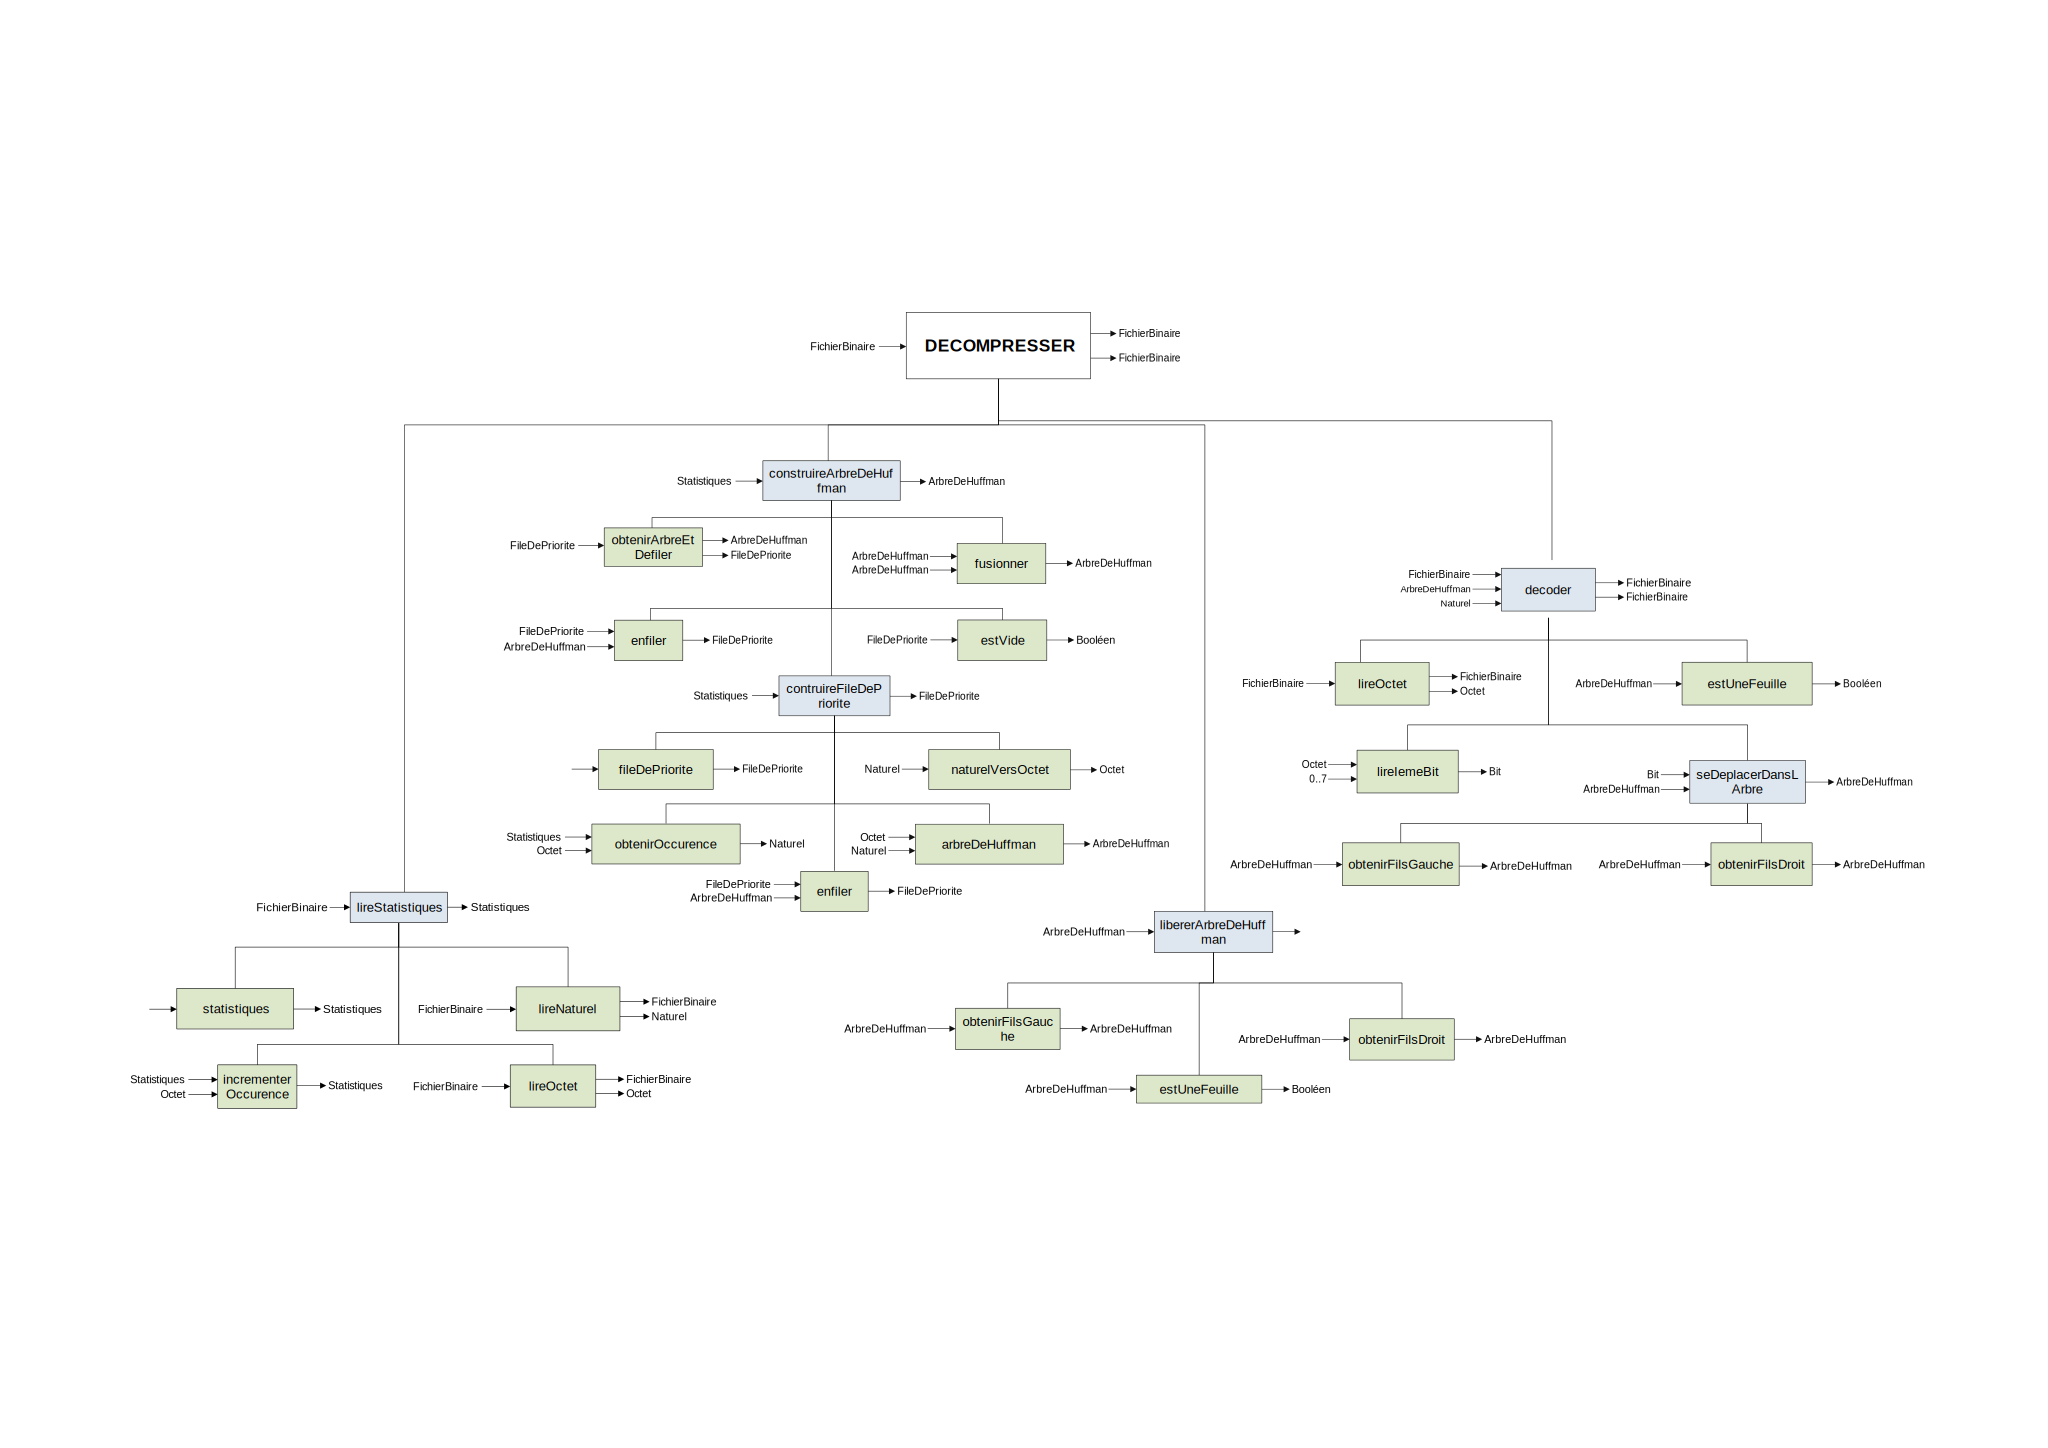
\includegraphics[width=1.1\textwidth]{images/decompresser.png}
    		\caption{Analyse descendante de la décompression}
    		\label{fig:exemple}
		\end{figure}
        \newpage
        \section{Conception Préliminaire}
        	\begin{algorithme}
    \signatureFonction{lireStatistiques}{f : \fichierbinaire}{\statistiques}{}
\end{algorithme}
        	\begin{algorithme}
    \signatureProcedure{decoder}
{\paramEntree{a : \arbredehuffman, longueur : \naturel}, \paramEntreeSortie{fb1 : \fichierbinaire, fb2 : \fichierbinaire}}{}
\end{algorithme}
        	\begin{algorithme}
    \signatureProcedure{libererArbreDeHuffman}
{\paramEntree{a : \arbredehuffman}}{}
\end{algorithme}
        	\begin{algorithme}
    \signatureProcedure{seDeplacerDansLArbre}
{\paramEntree{bit : \bit}, \paramEntreeSortie{arbreCourant : \arbredehuffman}}{}
\end{algorithme}

        \newpage
        \section{Conception Détaillée}
        	\begin{algorithme}
    \fonction{lireStatistiques}{fb : \fichierbinaire}{\statistiques}{}
    {naturelInutile, n, i : \naturel , s : \statistiques}
    {
		\sialors{non((estOuvert(fb)) et (mode(fb) $=$ lecture))}{    	
    		\instruction{ouvrir(fb, lecture)}
    	}
    	\\
    	\textcolor{gray}{//Lecture de l'identifiant (un \textit{unsigned long long int}) qui ici nous est inutile mais l'instruction permet de déplacer le curseur}
    	\instruction{lireNaturel(fb, naturelInutile)}
		\\
    	\textcolor{gray}{//Maintenant le curseur est au bon endroit et l'on peut lire les statistiques qui sont des \naturel}
    	\pour{i}{0}{255}{}
    	{
    		\instruction{lireNaturel(fb, n)}
        	\affecter{s[i]}{n}
    	}
    }
\end{algorithme}
        	\begin{algorithme}
\procedure{decoder}{\paramEntree{aHuff: \arbredehuffman}, \paramEntreeSortie{fb1 : \fichierbinaire}, \paramSortie{fb2 : \fichierbinaire}}{}{}
{
	\affecter{atemp}{aHuff}
	\tantque{non(finFichier(fb1))}
	{
		\affecter{OctetCourant}{lireOctet(fb1)}
		\pour{i}{0}{7}{}{
			\affecter{bit}{ObtenirIemebit(OctetCourant,i)}
			\instruction{seDeplacerDansArbre(atemp,bit)}
			\sialors{estUneFeuille(atemp)}{
				\affecter{octetDecodé}{obtenirOctet(arbreCourant)}
				\instruction{ecrireOctet(octetDecodé, fb2)}
				\affecter{aTemp}{aHuff}
				}
			}
		}
	}
\end{algorithme}
        	\begin{algorithme}
    \procedure{libererArbreDeHuffman}{\paramEntree{arbre : \arbredehuffman}}{}
    {
        \sialors{non estUneFeuille(arbre)}
        {
            \instruction{libererArbreDeHuffman(obtenirFilsGauche(arbre))}
          %  \instruction{libererArbreDeHuffman(obtenirFilsDroit(arbre))}
        }
       % \instruction{liberer(arbre)}
    }
\end{algorithme}
        	\begin{algorithme}
    \procedure{seDeplacerDansLArbre}{\paramEntree{bit : bit}, \paramEntreeSortie{arbreCourant : ArbreDeHuffman}}{}{}
    {
        \sialors{bit = 0}
        {
            \affecter{arbreCourant}{obtenirFilsGauche(arbreCourant)}
        }
        \sialors{bit = 1}
        {
            \affecter{arbreCourant}{obtenirFilsDroit(arbreCourant)}
        }
    }
\end{algorithme}

        	\begin{algorithme}
	\procedure{decompresser}{\paramEntreeSortie{fCompresse : \fichierbinaire}, \paramSortie{fDecompresse : \fichierbinaire}}
	{estOuvert(fCompresse) et (mode(fCompresse) $=$ lecture)}
	{i, id, longueur : \naturel, s : \statistiques, abh : \arbredehuffman, octetUnique : \octet}
    {
		\instruction{ouvrir(fDecompresse, ecriture)}
    	\instruction{positionnerAuDebut(fCompresse)}
    	\instruction{lireNaturel(fCompresser, id)}
		\\
    	\commentaire{On vérifie si on retrouve bien notre identifiant (ici 1000 sous sa forme de naturel), si ce n'est pas le cas, on n'a pas a décompresser le fichier}
    	\sialors{id = 1000}{   
			\instruction{lireNaturel(fCompresser, longueur)}
			\sialors{(longueur > 0)}{
				\instruction{lireStatistiques(fCompresser, s)}
				\instruction{construireArbreDeHuffman(s, abh)}
				\sialorssinon{estUneFeuille(abh)}
				{
					\affecter{octetUnique}{octetVersNaturel(obtenirOctet(abh))}
					\pour{i}{1}{longueur}{}{
						\instruction{ecrireOctet(octetUnique, fDecompresse)}
					}
				}
				{
					\instruction{decoder(abh, longueur, fCompresse, fDecompresse)}
				}
				\instruction{liberer(abh)}
			}
    	}
		\instruction{fermer(fDecompresse)}
    }
\end{algorithme}
        	\begin{algorithme}
	\fonction{construireArbreDeHuffman}{s : \statistiques}{\arbredehuffman}{}
	{fdp : \filedepriorite, dernierElement : \booleen, a1, a2, aFusion : \arbredehuffman}
    {
    	\affecter{fdp}{construireFileDePriorite(s)}
    	\affecter{dernierElement}{\textbf{Faux}}
    	\tantque{non(dernierElement)}
    	{
    		\instruction{obtenirElementEtDefiler(fdp, a1)}
    		\sialorssinon{estVide(fdp)}
    		{
    			\affecter{dernierElement}{\textbf{Vrai}}
    		}
    		{
    			\instruction{obtenirElementEtDefiler(fdp, a2)}
    			\affecter{aFusion}{fusionner(a1, a2)}
    			\instruction{enfiler(fdp, aFusion)}
    		}
    	}
    	\retourner{a1}
    }
\end{algorithme}
=======
        \section{Analyse descendante}
    \begin{minipage}{\textwidth}
        \includepdf{Ressources/AD_Decompresser.pdf}
    \end{minipage}
    
\newpage
\section{Conception Préliminaire}
    \begin{algorithme}
    \signatureFonction{lireStatistiques}{f : \fichierbinaire}{\statistiques}{}
\end{algorithme}
    \begin{algorithme}
    \signatureFonction{construireFileDePriorite}{s : \statistiques}{\filedepriorite}{}
\end{algorithme}
    \begin{algorithme}
    \signatureFonction{construireArbreDeHufmman}{s : \statistiques}{\arbredehuffman}{}
\end{algorithme}
    \begin{algorithme}
    \signatureProcedure{seDeplacerDansLArbre}
{\paramEntree{bit : \bit}, \paramEntreeSortie{arbreCourant : \arbredehuffman}}{}
\end{algorithme}
    \begin{algorithme}
    \signatureProcedure{decoder}
{\paramEntree{a : \arbredehuffman, longueur : \naturel}, \paramEntreeSortie{fb1 : \fichierbinaire, fb2 : \fichierbinaire}}{}
\end{algorithme}
    \begin{algorithme}
    \signatureProcedure{decompresser}{\paramEntreeSortie{fCompresse : \fichierbinaire}, \paramSortie{fDecompresse : \fichierbinaire}}{estOuvert(fCompresse) et (mode(fCompresse) $=$ lecture)}
\end{algorithme}

\newpage
\section{Conception Détaillée}
    \begin{algorithme}
    \fonction{lireStatistiques}{fb : \fichierbinaire}{\statistiques}{}
    {naturelInutile, n, i : \naturel , s : \statistiques}
    {
		\sialors{non((estOuvert(fb)) et (mode(fb) $=$ lecture))}{    	
    		\instruction{ouvrir(fb, lecture)}
    	}
    	\\
    	\textcolor{gray}{//Lecture de l'identifiant (un \textit{unsigned long long int}) qui ici nous est inutile mais l'instruction permet de déplacer le curseur}
    	\instruction{lireNaturel(fb, naturelInutile)}
		\\
    	\textcolor{gray}{//Maintenant le curseur est au bon endroit et l'on peut lire les statistiques qui sont des \naturel}
    	\pour{i}{0}{255}{}
    	{
    		\instruction{lireNaturel(fb, n)}
        	\affecter{s[i]}{n}
    	}
    }
\end{algorithme}
    \begin{algorithme}
    \fonction{construireFileDePriorite}{s : \statistiques}{\filedepriorite}{}
    {fdp : \filedepriorite, octet : \octet, occurence : \naturel}
    {
        \affecter{fdp}{fileDePriorite()}
        \pour{o}{ 0}{255}{}
        {
            \affecter{octet}{naturelVersOctet(o)}
            \affecter{occurence}{obtenirOccurence(s, octet)}
            \sialors{occurence > 0}{
                \instruction{enfiler(fdp, arbreDeHuffman(octet, occurence))}
            }
        }
        \retourner{fdp}
    }
\end{algorithme}
    \begin{algorithme}
	\fonction{construireArbreDeHuffman}{s : \statistiques}{\arbredehuffman}{}
	{fdp : \filedepriorite, dernierElement : \booleen, a1, a2, aFusion : \arbredehuffman}
    {
    	\affecter{fdp}{construireFileDePriorite(s)}
    	\affecter{dernierElement}{\textbf{Faux}}
    	\tantque{non(dernierElement)}
    	{
    		\instruction{obtenirElementEtDefiler(fdp, a1)}
    		\sialorssinon{estVide(fdp)}
    		{
    			\affecter{dernierElement}{\textbf{Vrai}}
    		}
    		{
    			\instruction{obtenirElementEtDefiler(fdp, a2)}
    			\affecter{aFusion}{fusionner(a1, a2)}
    			\instruction{enfiler(fdp, aFusion)}
    		}
    	}
    	\retourner{a1}
    }
\end{algorithme}
    \begin{algorithme}
    \procedure{seDeplacerDansLArbre}{\paramEntree{bit : bit}, \paramEntreeSortie{arbreCourant : ArbreDeHuffman}}{}{}
    {
        \sialors{bit = 0}
        {
            \affecter{arbreCourant}{obtenirFilsGauche(arbreCourant)}
        }
        \sialors{bit = 1}
        {
            \affecter{arbreCourant}{obtenirFilsDroit(arbreCourant)}
        }
    }
\end{algorithme}

    \begin{algorithme}
\procedure{decoder}{\paramEntree{aHuff: \arbredehuffman}, \paramEntreeSortie{fb1 : \fichierbinaire}, \paramSortie{fb2 : \fichierbinaire}}{}{}
{
	\affecter{atemp}{aHuff}
	\tantque{non(finFichier(fb1))}
	{
		\affecter{OctetCourant}{lireOctet(fb1)}
		\pour{i}{0}{7}{}{
			\affecter{bit}{ObtenirIemebit(OctetCourant,i)}
			\instruction{seDeplacerDansArbre(atemp,bit)}
			\sialors{estUneFeuille(atemp)}{
				\affecter{octetDecodé}{obtenirOctet(arbreCourant)}
				\instruction{ecrireOctet(octetDecodé, fb2)}
				\affecter{aTemp}{aHuff}
				}
			}
		}
	}
\end{algorithme}
    \begin{algorithme}
	\procedure{decompresser}{\paramEntreeSortie{fCompresse : \fichierbinaire}, \paramSortie{fDecompresse : \fichierbinaire}}
	{estOuvert(fCompresse) et (mode(fCompresse) $=$ lecture)}
	{i, id, longueur : \naturel, s : \statistiques, abh : \arbredehuffman, octetUnique : \octet}
    {
		\instruction{ouvrir(fDecompresse, ecriture)}
    	\instruction{positionnerAuDebut(fCompresse)}
    	\instruction{lireNaturel(fCompresser, id)}
		\\
    	\commentaire{On vérifie si on retrouve bien notre identifiant (ici 1000 sous sa forme de naturel), si ce n'est pas le cas, on n'a pas a décompresser le fichier}
    	\sialors{id = 1000}{   
			\instruction{lireNaturel(fCompresser, longueur)}
			\sialors{(longueur > 0)}{
				\instruction{lireStatistiques(fCompresser, s)}
				\instruction{construireArbreDeHuffman(s, abh)}
				\sialorssinon{estUneFeuille(abh)}
				{
					\affecter{octetUnique}{octetVersNaturel(obtenirOctet(abh))}
					\pour{i}{1}{longueur}{}{
						\instruction{ecrireOctet(octetUnique, fDecompresse)}
					}
				}
				{
					\instruction{decoder(abh, longueur, fCompresse, fDecompresse)}
				}
				\instruction{liberer(abh)}
			}
    	}
		\instruction{fermer(fDecompresse)}
    }
\end{algorithme}
>>>>>>> fa90880cec8105f32803241eaea2cc1967f219c1

    \chapter{Développement}
        \section{Fichiers d'en-tête}
    \subsection{TAD Octet}
        \inputminted[breaklines,fontfamily=lmss]{c}{../include/octet.h}
    \subsection{TAD Statistiques}
        \inputminted[breaklines,fontfamily=lmss]{c}{../include/statistiques.h}
    \subsection{TAD FileDePriorite}
        \inputminted[breaklines,fontfamily=lmss]{c}{../include/fileDePrioriteDArbreDeHuffman.h}
    \subsection{TAD ArbreDeHuffman}
        \inputminted[breaklines,fontfamily=lmss]{c}{../include/arbreDeHuffman.h}
    \subsection{TAD CodeBinaire}
        \inputminted[breaklines,fontfamily=lmss]{c}{../include/codeBinaire.h}
    \subsection{TAD TableDeCodage}
        \inputminted[breaklines,fontfamily=lmss]{c}{../include/tableDeCodage.h}
    \subsection{Construction de l'arbre de Huffman}
        \inputminted[breaklines,fontfamily=lmss]{c}{../include/construireArbreDeHuffman.h}
    \subsection{Compression}
        \inputminted[breaklines,fontfamily=lmss]{c}{../include/compression.h}
    \subsection{Décompression}
        \inputminted[breaklines,fontfamily=lmss]{c}{../include/decompression.h} 

\newpage
\section{Code source}
    \subsection{TAD Octet}
        \inputminted[breaklines,fontfamily=lmss]{c}{../src/octet.c}
    \subsection{TAD Statistiques}
        \inputminted[breaklines,fontfamily=lmss]{c}{../src/statistiques.c}
    \subsection{TAD FileDePriorite}
        \inputminted[breaklines,fontfamily=lmss]{c}{../src/fileDePrioriteDArbreDeHuffman.c}
    \subsection{TAD ArbreDeHuffman}
        \inputminted[breaklines,fontfamily=lmss]{c}{../src/arbreDeHuffman.c}
    \subsection{TAD CodeBinaire}
        \inputminted[breaklines,fontfamily=lmss]{c}{../src/codeBinaire.c}
    \subsection{TAD TableDeCodage}
        \inputminted[breaklines,fontfamily=lmss]{c}{../src/tableDeCodage.c}
    \subsection{Fonctions communes à la compression et à la décompression}
        \inputminted[breaklines,fontfamily=lmss]{c}{../src/construireArbreDeHuffman.c}
    \subsection{Compression}
        \inputminted[breaklines,fontfamily=lmss]{c}{../src/compression.c}
    \subsection{Décompression}
        \inputminted[breaklines,fontfamily=lmss]{c}{../src/decompression.c} 
    \subsection{Programme principal}
        \inputminted[breaklines,fontfamily=lmss]{c}{../src/main.c}

\newpage
\section{Tests unitaires}
    \subsection{Tests des TADs}
        \inputminted[breaklines,fontfamily=lmss]{c}{../src/testsTADs.c}
    \subsection{Tests des fonctions métier}
        \inputminted[breaklines,fontfamily=lmss]{c}{../src/testsFonctionsMetier.c}
                
<<<<<<< HEAD
        \chapter{Travail de Groupe}
        \begin{figure}[h] 
   			 \centering      
    		\includegraphics[width=1.1\textwidth]{images/TadTableau.png}
    		\caption{Tableau des tâches des TAD}
    		\label{fig:exemple}
		\end{figure}
		\begin{figure}[h] 
   			 \centering      
    		\includegraphics[width=1.1\textwidth]{images/compressionTableau.png}
    		\caption{Tableau des tâches de la compression}
    		\label{fig:exemple}
		\end{figure}
		\begin{figure}[h] 
   			 \centering      
    		\includegraphics[width=1.1\textwidth]{images/decompressionTableau.png}
    		\caption{Tableau des tâches de la décompression}
    		\label{fig:exemple}
		\end{figure}
        \chapter{Conclusion}
=======
    \chapter{Travail de Groupe}
        \section{Distribution des tâches}
    \begin{table}[ht]
    \centering
    \begin{tabular}{|c|c|>{\centering\arraybackslash}p{1.5cm}|>{\centering\arraybackslash}p{1.5cm}|>{\centering\arraybackslash}p{1.5cm}|>{\centering\arraybackslash}p{1.5cm}|}
        \cline{3-6}
        \multicolumn{2}{c|}{} & Taoba & Thomas & Ali & Mathis \\
        \hline
        \multirow{7}{*}{Analyse (TAD)}
        & CodeBinaire & & & $\times$ & \\
        \cline{2-6}
        & Octet & & & & $\times$ \\
        \cline{2-6}
        & Statistiques & $\times$ & & & \\ 
        \cline{2-6}
        & ArbreDeHuffman & & $\times$ & & \\
        \cline{2-6}
        & FileDePriorité & & $\times$ & & \\
        \cline{2-6}
        & TableDeCodage & & & & $\times$ \\
        \hline
        \multirow{7}{*}{CP}
        & Code Binaire & & & & $\times$ \\
        \cline{2-6}
        & Octet & & $\times$ & & \\
        \cline{2-6}
        & Statistiques & & $\times$ & & \\
        \cline{2-6}
        & ArbreDeHuffman & $\times$ & & & \\
        \cline{2-6}
        & FileDePriorité & & & & $\times$ \\
        \cline{2-6}
        & TableDeCodage & & & $\times$ & \\
        \hline
        \multirow{7}{*}{CD}
        & CodeBinaire & $\times$ & & & \\
        \cline{2-6}
        & Octet & $\times$ & & & \\
        \cline{2-6}
        & Statistiques & & & & $\times$ \\
        \cline{2-6}
        & ArbreDeHuffman & & & $\times$ & $\times$ \\
        \cline{2-6}
        & FileDePriorité & & & $\times$ & \\
        \cline{2-6}
        & TableDeCodage & & $\times$ & & \\
        \hline
        \multirow{7}{*}{Dev}
        & CodeBinaire & & $\times$ & & \\
        \cline{2-6}
        & Octet & & & $\times$ & \\
        \cline{2-6}
        & Statistiques & & $\times$ & & \\
        \cline{2-6}
        & ArbreDeHuffman & & & $\times$ & $\times$ \\
        \cline{2-6}
        & FileDePriorité & & & & $\times$ \\
        \cline{2-6}
        & TableDeCodage & $\times$ & & & \\
        \hline
        \multirow{7}{*}{Tests unitaires}
        & CodeBinaire & & $\times$ & & \\
        \cline{2-6}
        & Octet & & & $\times$ & \\
        \cline{2-6}
        & Statistiques & & $\times$ & & \\
        \cline{2-6}
        & ArbreDeHuffman & $\times$ & & & \\
        \cline{2-6}
        & FileDePriorité & $\times$ & & & \\
        \cline{2-6}
        & TableDeCodage & & & & $\times$ \\
        \hline
    \end{tabular}
    \caption{Tableau des tâches des TADs}
\end{table}

    \begin{figure}[h] 
        \centering      
        \includegraphics[width=1.1\textwidth]{compressionTableau.png}
        \caption{Tableau des tâches de la compression}
        \label{fig:exemple}
    \end{figure}

    \begin{figure}[h] 
            \centering      
        \includegraphics[width=1.1\textwidth]{decompressionTableau.png}
        \caption{Tableau des tâches de la décompression}
        \label{fig:exemple}
    \end{figure}

    \chapter{Conclusion}
        Conclusion

Dans ce projet, nous avons élaboré un algorithme de compression par perte basé sur un arbre de Huffman, en suivant une conception en quatre phase:

    La première phase a consisté en la conception des TADs (Types Abstraits de Données) et des analyses descendantes nécessaires à la mise en place de notre compresseur Huffman.

    Ensuite, nous avons réalisé la conception préliminaire de nos fonctions et procédures, jetant ainsi les bases de l'implémentation.

    La troisième phase a été consacrée à la conception détaillée, où nous avons approfondi chaque aspect de l'algorithme, clarifiant les spécifications et les interactions entre les différentes parties du code.

    Enfin, nous avons procédé à l'implémentation du code en langage C et à la réalisation des tests unitaires pour évaluer le fonctionnement des algorithmes.

Les résultats des tests, principalement réalisés sur des fichiers textes, démontrent l'efficacité de notre algorithme en termes de réduction de la taille des données, tout en préservant l'intégrité des informations d'origine.

L'utilisation d'une compression sans perte de données pour les fichiers texte est cruciale, car elle garantit la conservation du sens du texte d'origine. Nous aurions également pu explorer des méthodes de compression par perte de données et discuter de leur utilisation sur des fichiers audio ou images sur lesquels notre algorithme ne fonctionne pas étant des fichiers déjà compressé.

Le travail de groupe a été essentiel à la réussite de ce projet. Nous avons pu partager les tâches et les responsabilités, bénéficier des compétences et des connaissances des autres membres du groupe, et résoudre les problèmes de manière collective.

Concernant les perspectives d'amélioration, notre algorithme de compression pourrait être optimisé de différentes manières. Par exemple, l'utilisation d'un autre algorithme pour la construction de l'arbre de Huffman ou l'exploration de techniques de compression plus avancées telles que la compression par blocs ou la compression par transformation.




>>>>>>> fa90880cec8105f32803241eaea2cc1967f219c1
\end{document}
